% %This is a very basic article template.
% %There is just one section and two subsections.
\documentclass[authoryear, review,12pt,number]{elsarticle}
\usepackage[numbers]{natbib}
\usepackage{graphicx}
\usepackage{float}
\usepackage{rotating}
\usepackage{stfloats}
\usepackage{lineno}
\usepackage[linesnumbered,ruled,vlined]{algorithm2e}
\usepackage{tabulary}
\usepackage{graphicx}
\usepackage{color}
\usepackage[none]{hyphenat} \usepackage[table]{xcolor} \sloppy
\usepackage{hyperref}
\usepackage{amsmath}
\begin{document}

\begin{frontmatter}
\linenumbers
\title{Classifying EUNIS Habitats using Ontologies and Data Mining Methods}


\author[TUB]{T. Niklas Moran\corref{cor1}}
\ead{niklasmoran@mailbox.tu-berlin.de}

\author[TUB]{Simon Nieland}
\author[TUB]{Birgit Kleinschmit}

%\author[TUB]{Michael F\"orster}

\address[TUB]{Geoinformation in Environmental Planning Lab, Technische
Universit\"at Berlin, Stra\ss e des 17. Juni 145, 10623 Berlin, Germany}

\cortext[cor1]{Corresponding author at: Geoinformation in Environmental Planning
Lab, Technische Universit\"at Berlin, Stra\ss e des 17. Juni 145, 10623 Berlin,
Germany}  % el.:+49 30 314 72601;}

\begin{abstract}
Remote sensing Biodiversity monitoring and 
\end{abstract}

\begin{keyword}
remote sensing, biotope classification, data mining,
generalisation, nature conservation, OWL, EUNIS, OBIA
\end{keyword}

\end{frontmatter}

\linenumbers

\section{Introduction}  % NATURA2000 obligations and local obligations = NATFLO
Recognizing that the decreasing number of
intact habitats in Europe  plays a dominant role in biodiversity loss, the
European Union has implemented an environmental conservation framework to halt
biodiversity loss in accordance with the Convention on Biological Diversity
(CBD, 2005). An integral part of this framework is the EU Habitats Directive
(Council Directive) 92/43/EEC [1992], which established the Natura 2000 network
of habitats. The law requires conservation and monitoring of designated habitats
by member states and for a report to be submitted every six years.
Environmental data to determine biodiversity status must be collected to comply
with the statute. Yet, comparing data used for these reports can be
difficult due to varying data collection methods by the nature conservation
authorities in each member state \citep{INSPIREdataspecs, INSPIRE}.
The main issue lies in the subjective nature of field surveys to identify
habitats \citep{Cherrill1999, Cherrill1999a, Nieland2015} and  %Nieland2016
complicating matters further, habitat status is mostly generated in
bottom-up approaches taking into account the national and regional
interpetation guidelines \citep{INSPIREdataspecs}. Using remote sensing
data could help address some of these issues.
\\
Remote sensing (RS) combined with Object-Based Image Analysis (OBIA), which
segments the image into homogenous image objects \citep{Blaschke2010}, offers
opportunities to automate and collect large amounts of computer-readable data
useful for nature conservation and biodiversity monitoring \citep{Corbane2015,
VandenBorre2011, Mayer2011}. Yet, RS image analysis implicitly incorporates the
expertise and knowledge of the person performing the analysis and reduces
objectivity. This can be divided into remote sensing knowledge (spectral
signature, remote sensing index, etc.) and field knowledge (feature properties,
spatial relations, etc) \citep{Andres2013a}. This knowledge is often neither
completely nor explicitly defined but influences the classification. To ensure
accuracy and applicability of classification outputs for conservation, experts
with detailed knowledge of the sites are needed to interpret the EO data. To
alleviate this problem, ontologies can foster data exchange and reuse by
formalizing knowledge with standardized languages such as OWL. The developed
terms can be imported and combined with other terms available on the Linked Data
Cloud.
\\
While different fields (medical imaging, security, etc.) have used ontologies,
only recently have ontologies been adopted in remote sensing research. An
ontology, defined  as ``an explicit specification of a conceptualization''
\citep{gruber1993} could help bridge the semantic gap and allow for better data
transferability, reproducability, interoperability, knowledge and workflow
management and logical consistency. Moreover, through the use of reasoners
(inference engines) that infer logical consequences over axioms and asserted 
facts one can discover new knowledge \citep{Arvor2013, Andres2013a}. The term
``semantic gap'' refers to the difference between the higher-level descriptions
by experts and what can be extracted from the visual data. RS and
field expert knowledge can be digitized in ontologies, thus allowing for a
hierarchy of concepts for improved automatic image annotation and retrieval
using concepts from both fields to produce more accurate results
\cite{Srikanth:2005:EOA:1076034.1076128}. Janowicz \cite{Janowicz2012} advocates
for more observation-driven ontologies and for including machine learning,
geostatistics and data mining to construct ontological primitives. While
research on using observation-based ontologies for classifications is limited,
the available research in RS using ontologies is briefly summarized below.
\\
The EU-funded ``Biodiversity Multi-Source Monitoring System: From Space To
Species'' (BIO\_SOS) project seeks to develop tools to monitor and map protected
areas in the EU and uses ontologies modeled on the Land Cover Classification
System (LCCS) and the General Habitat Category (GHC) to achieve this goal
\citep{Arvor2013}. Using the taxonomy of the different classification systems
allows expert knowledge to be included in the process. Further work as part of
the project includes creation of a standardized
framework for habitat monitoring and mapping called the Earth Observation Data
for Habitat Montioring (EOD-HAM) system \citep{Lucas2015}. The system harnesses
knowledge from both remote sensing and ecology to classify Natura 2000 sites
using a hierarchical classification system. The EOD-HAM system uses both
pixel-based analysis and OBIA for greater classification accuracy but still
relies on a rule-base created by an expert. Other research includes
classification of urban building types using a three-layered architecture
\citep{diSciascio2013} and a semi-automated classification of urban building
using the Random Forest (RF) classifier to determine variable importance of
features from airborn laser scanner data \citep{Belgiu2014}. Ontologies have
also been paired with different algorithms to automatically acquire
classification rules: a genetic programming algorithm
\citep{Forestier2012470} and the C4.5 data mining algorithm
\citep{Sheeren2006ML}. Harnessing ontologies to improve spatial data
interoperability has been demonstrated by using ontological inference and
hierarchical matchmaking by Nieland et al. \citep{Nieland2015}. 
\\
Even though researchers recently developed a number of indicators using
different sensors for habitat evaluation \citep{Nagendra2013}, classification
procedures and rulesets were not formalised to be computer readable and
therefore suffer from similar transferablity and reproducablity problems as
manual habitat mapping \citep{Arvor2013, Nieland2015}.
Therefore a formalized computer-readable ontology could help solve these
problems and allow scientists to see how the classification was performed and be
more aware of possible incompatibilities before combining datasets
\citep{Janowicz2012}. 
Furthermore, there is no standardized set of indicators
using RS for trans-national habitat evaluation \citep{Lucas2015}. Therefore,
technical solutions to increase interoperability by thematically harmonizing
environmental data and systematize data collection methods from remote sensing
inputs in an automated workflow would allow decision-makers to better assess and
compare outcomes.
\\
In this paper we propose an automated system that can
classify selected biotopes according to the European Union Nature Information
System (EUNIS) biotope classification schema using EO data, existing
thematic maps (biotope, forestry, etc.) and expert knowledge formalized in an
ontology. The biotope indicators serve as class labels for training data mining
algorithms which generate rules that can be imported into an ontology. Once the
rules and segmented objects are imported into the ontology, a reasoner can
perform reasoning classifying which objects belong to which class and how the
classes are related. The combination of data mining algorithms with
ontology-based classification has not yet been done and is a first in remote
sensing research. This method contributes to the goal of empirically-derived
rule creation and enhances data interoperability and comparison as proposed by Janowicz 
\citep{Janowicz2012}.
%Arvor2013. Was ist Reasoning?  Du musst auch noch erklären was data mining/
%machine learning ist und die in der Fernerkundung gängigsten Algorithmen
%erwähnen (SVM, RF, BRT, DT) Bitte alle mit Quelle!
% Wichtig ist, dass du nochmal ganz explizit die Innovation deines Papers
% hervorhebst. 
%Die kombination von Data Mining algorithmen und ontologiebasierter
%Klassifikation gibt es bislang in der Fernerkundung noch nicht. Schreib das so
%hin! Schreib genau was die anderen bislang gemacht haben und was du jetzt noch
%zus\a'tlich ergnzt hast (im Bezug auf Belgiu usw.).
\section{Method}
\subsection{Target indicators and base nomeclatures}
We test our method on EUNIS E1- dry, E2- mesic and E3- wet
grasslands. The table below describes the indicators that are needed to identify
and hence classify the biotopes according to the EUNIS classification hierachy.
\label{tab_indicators_classes}
% Bitte beschreibe genau welche Klassen du ableiten willst und welche
% Indikatoren du daf�r ben�tigst (vielleicht in einer Tabelle). Du kannst auch
% etwas �ber die Hierarchische Struktur und den nach Indikatoren gegliederten
% Aufbau von EUNIS schreiben. Schreib, dass wir die Indikatoren aus EUNIS
% �bernommen haben und auf die Anforderungen fernerkundlicher Analysen angepasst
% haben. Nach M�glichkeit haben wir uns and der EAGLE nomenclature orientiert
% um eine �bergeordnete interoperablit�t zu gew�hrleisten.

\label{subsec_indicators_and_nomenclatures}
\subsection{Overview of the Automated EUNIS Habitat Mapping System}
% EU-HMS?
This section describes the developed method for classifying EUNIS habitats by
using data mining algorithms to generate rules based on remote sensing, digital
surface model (DSM) and digital terrain model (DTM) derived statistics of
pre-segmented polygons. The method's use of ontologies and the advantage
theirein is also explained.\\
The system is comprised of (1) attaching
formalized habitat indicators from expert knowledge to pre-segmented polygons,
(2) rule generation by running data mining algorithms over randomly selected
polygons and using the habitat indicators as class labels, (3) importing rules,
EUNIS classes and polygon attributes into an ontology and finally (4)
classifying polygons with the Fact++ reasoner \citep{Tsarkov2006} and writing results back
to the database. An overview of the complete workflow is shown in figure
\ref{fig_full_workflow}.\\
The software relies on a PostgreSQL database backend with PostGIS extensions
enabled and various open source Python and Java libraries to interact with the
database, convert files and execute a reasoner over the created OWL file.
SQLAlchemy is used for database interaction and data management is done with
the Python Data Analysis Library (Pandas) \citep{McKinney2010}. The OWLAPI is
used to interact with the OWL files and execute the FaCT++ reasoner
\citep{Tsarkov2006}. The software is freely available and is released under an
open source license.  
\begin{figure}
    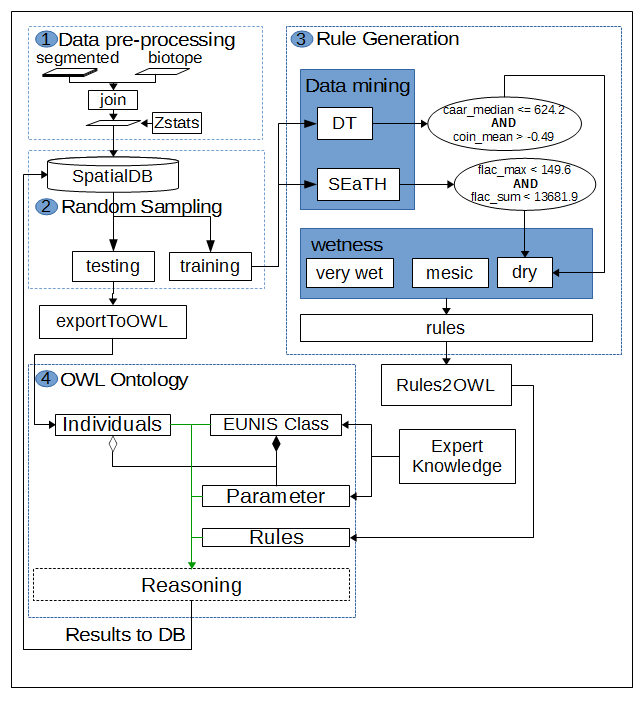
\includegraphics[width=1\linewidth]{diagrams/another_workflow_diagram_large.png}
    \caption
    {
        1) The thematic maps (biotope, forestry, etc.) are joined together and
        statistics are calculated for each combined polygon.
        2) Training and testing data are created and saved in the database.
        3) The training data is loaded into the data mining module and the
        rules are generated for the ``wetness" indicator
        4) The rules are imported into the OWL ontology along with the testing
        data as individuals. The reasoner performs A-box reasoning to determine
        class membership.
    } 
\label{fig_full_workflow}
\end{figure}
\subsection{Formalization of Expert Knowledge}
EUNIS class descriptions and interpretation guidelines \citep{EUNISManual} were
used to develop a set of indicators to accurately formalize certain habitats
with regard to the inferability with available input data sets (see
\ref{subsec_indicators_and_nomenclatures}). This formalisation can then be
written to an OWL ontology, which is able to store complex logical connections
in a XML based data structure. The goal is to produce what Janowicz describes
as a ``microtheory'' \citep{Janowicz2012} which can then be used to map other
theories by training the data mining algorithms for the new
region and using the reasoner. We use environmental variables (e.g., surface
wetness, slope position) from the classification schemes and concepts from
EAGLE to create a comprehensive interoperable vocabulary. This process involved
attaching indicators from EUNIS, newly created indicators by NATFLO and EAGLE
to each biotope. For example, the parameter ``wetness'' could be any of
``aquatic", ``dry'', ``mesic", ``moist" or ``very wet''. An example of
a EUNIS class, E2.22 ``Sub-Atlantic lowland hay meadows'' modeled with selected
remote sensing indicators is written in description logic (DL) below:
%\begin{equation}
\begin{align*}
%\begin{split}
E2.22 &\equiv water\_regime \exists \{``intermittent\_desiccation''\} \\
&\qquad {} \land acidity \exists \{``acid''\} \\
&\qquad {} \land geological_characteristics \exists \{``siliceous''\}\\
&\qquad {} \land usage \exists \{``mowing''\} \\
&\qquad {} \land usage\_intensity \exists \{``high''\} \\
&\qquad {} \land wetness \exists \{``mesic''\} \\
\end{align*}
\subsection{Rule Generation with Data Mining}
The data mining module randomly selects polygons for training and testing from
the database and applies the selected algorithm on the training data. 
%
Currently the data mining module uses the decision tree classifier from
scikit-learn \citep{scikit-learn} and the Separability and Thresholds (SEaTH)
algorithm \citep{Nussbaum2006} but the method can be extended to use other
algorithms as long as the algorithm can generate a ruleset that can be
converted to OWL. In the next step the rules can be imported into an OWL
ontology along with the testing data. In the last step the reasoner (FaCT++)
classifies all polygons according to the rules and writes the results to the
database (see figure \ref{fig_full_workflow}.
\\
We chose supervised classification algorithms that
are able to exploit expert knowledge, perform classification tasks quickly and
accurately and produce human understandable rule sets for further scrutiny and
refinement. Therefore, the SEaTH algorithm and the decision tree classifier
(DT) were selected to find the optimal combination of environmental indices and
object properties that differentiate between objects. To compare classification
accuracy we selected the scikit-learn Python suite \citep{scikit-learn} due to
its maturity, ease of use and the availability of different algorithms. 

%\subsection{SEaTH}
The Separability and Thresholds (SEaTH) algorithm \citep{Nussbaum2006}
statistically identifies characteristic features and their thresholds. It has
been used on remote sensing data for land cover classification \citep{Gao2011}
and nuclear installation classification \citep{Nussbaum2006}. Using training
data, the algorithm determines the separability of the object classes and then
calculates the thresholds for which the maximum separability can be achieved
using the given features. One benefit of the algorithm is that one does not
need many training objects.  In  \cite{Nussbaum2006}, for example, the authors
suggest using only very characteristic features for training and only used
around 10 samples per class. The authors also state that usually two features
per class is enough to produce accurate results.\\

%\subsection{Decision Tree Classifier}
The decision tree (DT) classifier implemented in scikit-learn is a modified
classification and regression tree (CART)\citep{scikit-learn}. The extra trees
(ET) classifier is a modified random forest without bootstrapping and instead of
splitting on the most discriminative feature, random thresholds from candidate
features are taken.
An evolutionary search algorithm based on the Distributed Evolutionary
Algorithms in Python (DEAP) \citep{DEAP_JMLR2012} software searches
for the best parameters for both the DT and ET classifiers. The evolutionary
search cross-validation method was much quicker than the grid search cross
validation. 
%Then the rules generated by the algorithm is converted with an automated
%Python script to OWL Ontology rules. Hier fehlt der Bezug
\subsection{Segmentation} 
\label{subsec_segmentation}
The iterative object-based image analysis is performed using Defiens eCognition
Server and segments the data using thresholds and multi-resolution approaches
(Baatz and Sch\'ape 2000). The segmentation process uses information solely from
aerial images based on spectral information (NDVI and Bare Area Index) and
height from the digital elevation model (DEM) to separate between biotic and
no-biotic features \citep{Tintrup2015}. The detailed pre-processing workflow is
shown in figure \ref{fig_pre-processing}.
\subsection{Benefits of using an ontology}
RS image analysis implicitly incorporates the expertise and
knowledge of the person performing the analysis and reduces objectivity. This
can be divided into remote sensing knowledge (spectral signature, remote
sensing index, etc.) and field knowledge (feature properties, spatial
relations, etc) \citep{Andres2013a}. This knowledge is often neither completely
nor explicitly defined but influences the classification. To ensure accuracy and
applicability of classification outputs for conservation, experts with detailed
knowledge of the sites are needed to interpret the EO data. To alleviate this
problem, ontologies can foster data exchange and reuse by formalizing knowledge
with standardized languages such as OWL. The developed terms can be imported and
combined with other terms available on the Linked Data Cloud. 
\section{Data and Study Area}
All input data comes from the RLP Ordnance Survey (Landesamt f\"ur Vermessung 
und Geobasisinformation). The data is segmented by RLP AgroScience using
multi-spectral (B, G, R, NIR) orthophotos with a 0.2m ground resolution and a
2 x 2km tile size. The orthophotos are updated every 2 years and are used to
create the Digital Surface Model (DSM) using automated stereo matching. The
last available orthophotos are from 2013. The DTM and
DEM was produced using LiDAR ASCII point clouds acquired between 2003 and 2009
with a resolution of 0.5m.\\
\subsection{Segmentation}
The iterative object-based image analysis is performed using Defiens eCognition
Server and segments the data using thresholds and multi-resolution approaches
(Baatz and Sch\'ape 2000). The segmentation process uses information solely
from aerial images based on spectral information (NDVI and Bare Area Index) and
height from the digital elevation model (DEM) to separate
between biotic and no-biotic features \citep{Tintrup2015}. T 
The detailed pre-processing workflow is shown in figure
\ref{fig_pre-processing}.
\subsection{Segmentation} The iterative object-based image analysis is
performed using Defiens eCognition Server and segments the data using
thresholds and multi-resolution approaches (Baatz and Sch\'ape 2000). The
segmentation process uses information solely from aerial images based on
spectral information (NDVI and Bare Area Index) and height from the digital
elevation model (DEM) to separate between biotic and no-biotic features
\citep{Tintrup2015}. The detailed pre-processing workflow is shown in figure
XX.
%EAGLE nomenclature for landcover classes.
\subsection{Thematic Maps} The RLP biotope map was last updated in 2015. The
agriculture data set (INVEKOS) is updated yearly. The Forestry map is from:
200X and the soil map is from 200X.

\begin{figure} 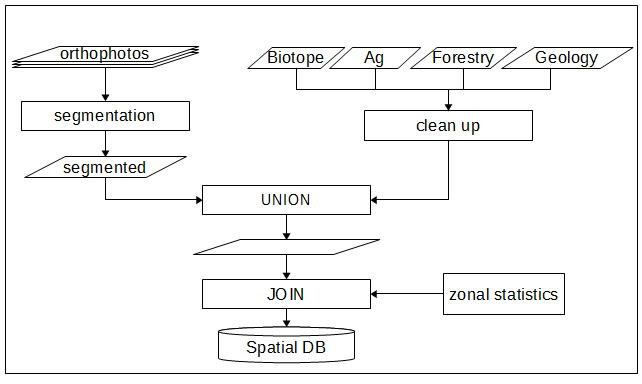
\includegraphics[width=1\textwidth]{diagrams/pre_processing.png}
    \caption{Biotope, Agriculture, Forestry, Geology (soil maps) are unioned to
    then be joined by the segmented polygons derived from orthophotos. The
    features are joined together and get all properties associated from the
    dataset unless they conflict. When conflicts occur the corresponding column
    is marked as such.}
\label{fig_pre-processing}
\end{figure}
To compare classification accuracy we selected the scikit-learn Python suite
\citep{scikit-learn} due to its maturity and ease of use and the availability of
different algorithms. One can visualize the results and parse the tree to load
the results into the ontology.

\subsection{Study Area and Data}
%% southwestern?!
All input data comes from the RLP Ordnance Survey (Landesamt f\"ur Vermessung
und Geobasisinformation). The data is segmented by RLP AgroScience using
multi-spectral (B, G, R, NIR) orthophotos with a 0.2m ground resolution and a 2
x 2km tile size. The orthophotos are updated every 2 years and are used to
create the Digital Surface Model (DSM) using automated stereo matching. The
last available orthophotos are from 2013. The DTM and DEM was produced using
LiDAR ASCII point clouds acquired between 2003 and 2009 with a resolution of
0.5m.\\
%rapid eye daten einbeziehen. mach doch vielleicht eine Tabelle. Das spart
%Platz.
Saarburg is an 200km$^{2}$ administrative district and is located in the
south-west of the federal state of Rhineland Palatinate (RLP), Germany.
Luxembourg borders the area to the west and the federal state of Saarland to
the South.  RLP has a western european atlantic climate and has an economically
and culturally important viticulture industry along the Mosel and Rhine rivers.
\begin{figure}
\label{fig_study_area}
    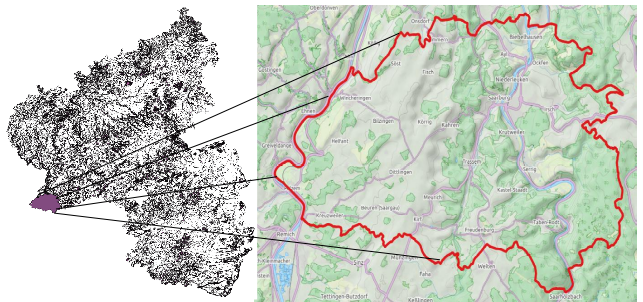
\includegraphics[width=\textwidth]{diagrams/study_area_closeup.png}
    \caption{The location of Saarburg on the left in purple in relation to
    Rheinland Palatinate. Map on right \copyright Thunderforest, Data
\copyright OpenStreetMap contributors.}
\end{figure}

\subsection{Validation} 
The data was divided into 20\% for training and 80\% for validation. For SEaTH
20 objects per class were used from the training data set because the algorithm
performs better with a smaller number of features \citep{Nussbaum2006}. 
\section{Results}
Training  the data with the ET classifier yielded classification results of
100\% for indicators usage, wetness and depression.

\section{Discussion} SEaTH shows much better separability when one chooses
larger objects and fewer training objects per class. Training SEaTH on a few
carefully selected objects being ideal class representations further increases
the separability, but the classification accuracy suffers when applied to the
complete data set. Thus, SEaTH appears to over-fit. Using two sets of rules
produced from different sized training data produced quite different results
when tested on the same dataset.
\section{Conclusion} We showed an automated
workflow using ontologies and data mining algorithms can accurately classify
EUNIS habitat objects. Moreover, the use of ontologies if published on the
Internet can allow others to reuse the workflow and make their own
modifications. 
\section{Acknowledgments}
We would like to thank RLP AgroScience GmbH for processing the data and the
RLP's Environment Ministry for funding the  NATFLO project. This work was
conducted using the Prot\'eg\'e resource, which is supported by grant GM10331601 from the
National Institute of General Medical Sciences of the United States National
Institutes of Health.
\bibliographystyle{model2-names}
\section{References} \bibliography{references} \end{document}
